%!TEX root = ./template-skripsi.tex
%-------------------------------------------------------------------------------
%                            	BAB IV
%               		UJI COBA DAN HASIL UJI COBA
%-------------------------------------------------------------------------------

\chapter{UJI COBA DAN HASIL UJI COBA}

\section{Uji Coba}
Pada bagian ini akan dijelaskan mengenai pengujian Sistem Informasi \textit{Tracer Study} Program Studi Ilmu Komputer yang telah dikembangkan. Sesuai dengan tahapan SDLC \textit{spiral model} setelah tahapan konstruksi atau pengembangan akan dilanjutkan ke tahapan evaluasi atau pengujian. Tahapan ini bertujuan untuk memastikan sistem yang telah dibuat dapat bekerja sesuai dengan kebutuhan, memperoleh umpan balik dari pengguna, dan menemukan kesalahan atau \textit{bugs} pada sistem. 

Uji coba pada sistem dilakukan tehadap satu responden ahli untuk uji keseluruhan sistem, satu reponden admin, satu responden koorprodi, 15 responden alumni, dan 5 responden pengguna alumni. Setiap responden akan melakukan pengujian terhadap sistem berdasarkan peran masing-masing responden. Uji coba yang dilakukan menggunakan kuesioner Pengujian Penerimaan Pengguna atau yang disebut dengan UAT (\textit{User Acceptance Test}). Langkah-langkah pengujian Sistem Informasi \textit{Tracer Study} Prodi Ilmu Komputer adalah sebagai berikut. 

\begin{enumerate}
	\item Admin mengelola (menambah, menyunting, menghapus) data alumni. 
	\item Admin menyunting kata pengantar untuk beranda alumni
	\item Admin membuat kuesioner untuk alumni dan pengguna alumni
	\item Alumni menyunting profil atau data diri
	\item Alumni mengelola  (menambah, menyunting, menghapus) riwayat pekerjaan. 
	\item Alumni mengisi kuesioner yang dibuat admin
	\item Admin mengelola (menambah, menyunting, menghapus) data pengguna alumni.
	\item Pengguna alumni mengisi kuesioner yang dibuat admin
	\item Admin melihat laporan hasil \textit{tracer study}
	\item Koorprodi melihat data alumni dan pengguna alumni
	\item Koorprodi melihat laporan hasil \textit{tracer study}
\end{enumerate}

Pengujian pada sistem ini terdiri dari dua, yaitu pengujian fungsional dan kebergunaan atau \textit{usability}. Pengujian fungsional berfokus pada fungsionalitas perangkat lunak yang dikembangkan. Sedangkan pengujian kebergunaan dilakukan untuk mengukur kegunaan sistem dan kemudahan penggunaan sistem dalam membantu pengguna memenuhi kebutuhannya. Berikut adalah komponen-komponen yang akan diuji pada Sistem Informasi \textit{Tracer Study} Prodi Ilmu Komputer:

\begin{enumerate}
	\item Admin
	\begin{itemize}
		\item Mengelola (menambah, menyunting, menghapus) data alumni
		\item Mengelola (menyunting dan menghapus) data pengguna alumni
		\item Menyunting kata pengantar \textit{tracer study}
		\item Membuat kuesioner alumni dan pengguna alumni
		\item Melihat laporan hasil \textit{tracer study}
	\end{itemize}
	\item Kooprodi
	\begin{itemize}
		\item Melihat data alumni
		\item Melihat data pengguna alumni
		\item Melihat laporan hasil \textit{tracer study}. 
	\end{itemize} 
	\item Alumni
	\begin{itemize}
		\item Menyunting data diri dan mengelola riwayat pekerjaan
		\item Mengisi form kuesioner \textit{tracer study}
		\item Melihat daftar pengguna alumni beserta alumni yang bekerja
	\end{itemize} 
	\item Pengguna Alumni
	 \begin{itemize}
	 	\item Mengisi form kuesioner pengguna alumni
	 \end{itemize}
\end{enumerate}
Dari semua komponen penilaian tersebut untuk pengujian fungsional dilakukan
dengan dua pilihan yaitu :
\begin{enumerate}
	\item S  : Setuju
	\item TS : Tidak Setuju
\end{enumerate}
Sedangkan untuk pengujian kebergunaan (\textit{usability}) dilakukan menggunakan skala \textit{likert}. Skala \textit{likert} merupakan 
suatu skala penilaian yang menyajikan pilihan skala dengan nilai pada setiap skala untuk mengukur tingkat persetujuan terhadap sesuatu \cite{Maryuliana}.  Skala yang digunakan dengan nilai 1 sampai 5 dengan perincian sebagai berikut :
\begin{itemize}
	\item 1 : Sangat Tidak Setuju
	\item 2 : Tidak Setuju
	\item 3 : Cukup
	\item 4 : Setuju
	\item 5 : Sangat Setuju
\end{itemize}

Berdasarkan nilai yang didapatkan dari pengguna saat pengujian, angka tersebut akan dikalkulasikan sesuai dengan sistem penilaian berikut :

\begin{itemize}
	\item Nilai total
	
	Nilai total merupakan jumlah keseluruhan nilai/skor yang didapat pada setiap pertanyaan atau dapat ditulis menjadi:
	
	$Nilai$ $Total = (jumlah \times skor SS) + (jumlah \times skor S) + (jumlah \times skor C) + (jumlah \times skor TS) + (jumlah \times skor STS)$ 
	
	\item Persentase Kelayakan
	
	Presentase kelayakan atau persentase nilai rata-rata yang didapatkan dari nilai total dibagi skor yang diharapkan. Skor yang diharapkan didapat dari skor maksimal yang dikalikan dengan jumlah responden. Skor maksimal adalah nilai maksimal dari skala \textit{likert} dikalikan dengan jumlah pertanyaan. Perhitungan tersebut dapat ditulis menjadi :
	
	$Persentase$ $Kelayakan (\%) = $ $\frac{Nilai Total}{Skor Diharapkan}$ $\times 100\%$

\end{itemize}

Persentase kelayakan yang didapatkan akan dibandingkan dengan skor pada skala \textit{likert}. Berikut model skala \textit{likert} lima skala :
\begin{enumerate}
	\item Sangat Kurang Sesuai = 0\%-20\%
	\item Kurang Sesuai = 21\%-40\%
	\item Cukup Sesuai = 41\%-60\%
	\item Sesuai = 61\%-80\%
	\item Sangat Sesuai = 81\%-100\%
\end{enumerate}

\section{Hasil Percobaan}
Berdasarkan percobaan yang dilakukan terhadap 1 admin, 1 koorprodi, 15 alumni, dan 5 pengguna alumni, didapatkan hasil percobaan sebagai berikut :

\subsection{Pengujian oleh Admin}
Pengujian untuk \textit{user} admin dilakukan oleh seorang responden yang bernama Bapak Alfisyahrizqa selaku staf admin prodi Ilmu Komputer pada tanggal 8 Januari 2020. Penilaian yang diberikan seputar fungsionalitas dan kebergunaan dari halaman \textit{user} admin pada sistem \textit{tracer study} Ilmu Komputer

\begin{enumerate}
	\item Uji Coba Fungsional
	
	Tabel 4.1 adalah hasil uji fungsional pada admin \textit{tracer study} :
	
	\begin{table}[H]
		\centering
		\caption{Hasil Uji Fungsional pada \textit{user} Admin}
		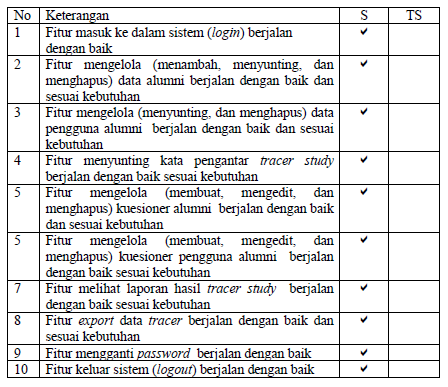
\includegraphics[width=10cm,height=9cm]{gambar/UAT/f_admin}
		\label{f_admin}
	\end{table}

Berdasarkan hasil uji coba fungsional yang dilakukan, keseluruhan fitur \textit{user} admin pada  sistem informasi \textit{tracer study} prodi Ilmu Komputer dapat berjalan dengan baik dan sesuai dengan yang diharapkan.
	
	\item Uji Coba Kebergunaan
	
	Berikut merupakan daftar pertanyaan uji \textit{usability} pada Admin:
	
	\begin{table}[H]
		\centering
		\caption{Daftar Pertanyaan Uji \textit{Usability} pada Admin}
		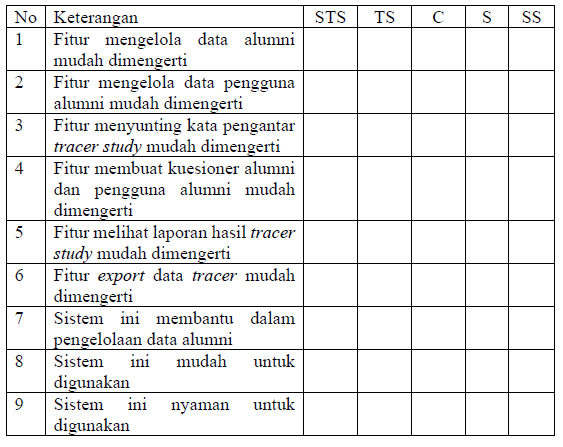
\includegraphics[width=11cm,height=10cm]{gambar/UAT/u_admin}
		\label{u_admin}
	\end{table}
	
	Berikut merupakan hasil uji kebergunaan pada admin \textit{tracer study} yang dapat dilihat pada tabel berikut:
	
	\begin{table}[H]
		\centering
		\caption{Hasil uji \textit{usability} pada Admin}
		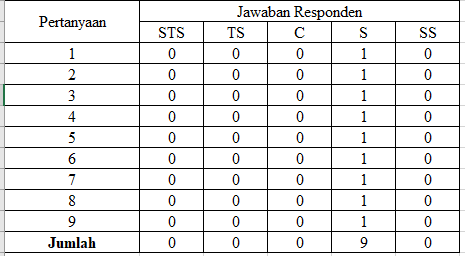
\includegraphics[width=12cm,height=7cm]{gambar/UAT/hasil_u_admin}
		\label{h_u_admin}
	\end{table}
	
	$Nilai$ $Total = (0 \times 1) + (0 \times 1) + (0 \times 3) + (9 \times 4) + (0 \times 5) = 36$
	
	$Persentase$ $kelayakan (\%) = \frac{36}{45} $ $\times 100\%$ = 80\%
	
	Berdasarkan hasil uji coba kebergunaan yang telah dilakukan, didapatkan persentase kelayakan senilai \textbf{80\%}. Maka dapat dikatakan halaman pada \textit{user} admin mendapatkan predikat sesuai untuk aspek kebergunaan sistem. Dengan catatan data pada sistem di-\textit{update} dengan data terbaru.
	
\end{enumerate}

\subsection{Pengujian oleh Koorprodi}
Pengujian untuk \textit{user} koorprodi dilakukan oleh seorang responden yang bernama Ibu Ir. Fariani Hermin I, M.T. selaku koorprodi Ilmu Komputer pada tanggal 8 Januari 2020. Penilaian yang diberikan terkait fungsionalitas dan kebergunaan dari halaman \textit{user} koorprodi pada sistem tracer study Ilmu Komputer.

\begin{enumerate}
	\item Uji Coba Fungsional
	
	Tabel 4.4 adalah hasil uji fungsional pada koorprodi :
	
	\begin{table}[H]
		\centering
		\caption{Hasil Uji Fungsional pada Koorprodi}
		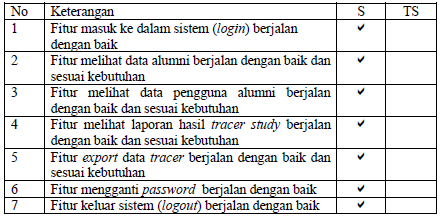
\includegraphics[width=11cm,height=7cm]{gambar/UAT/f_koorprodi}
		\label{f_koorprodi}
	\end{table}
	
	%lihat lg hasil real nya/jelasin
	Berdasarkan hasil uji coba fungsional yang dilakukan, sistem informasi
	\textit{tracer study} prodi Ilmu Komputer dapat berjalan dengan baik dan sesuai dengan yang dibutuhkan. Koorprodi Ilmu Komputer dapat melihat data alumni dan pengguna alumni, dapat melihat laporan hasil \textit{tracer study}, dan \textit{export} data \textit{tracer}.
	
	\item Uji Coba Kebergunaan
	
	Berikut merupakan daftar pertanyaan uji \textit{usability} pada Koorprodi:

	\begin{table}[H]
		\centering
		\caption{Daftar Pertanyaan Uji \textit{Usability} pada Koorprodi}
		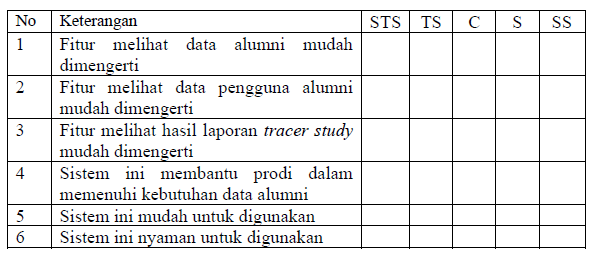
\includegraphics[width=11cm,height=7cm]{gambar/UAT/u_koorprodi}
		\label{u_koorprodi}
	\end{table}
	
	Berikut merupakan hasil uji \textit{usability} pada koorprodi yang dapat dilihat pada tabel berikut:
	
	\begin{table}[H]
		\centering
		\caption{Hasil Uji \textit{Usability} pada Koorprodi}
		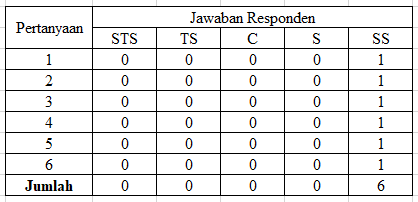
\includegraphics[width=11cm,height=8cm]{gambar/UAT/hasil_u_koorprodi}
		\label{h_u_koorprodi}
	\end{table}
	
	$Nilai$ $Total = (0 \times 1) + (0 \times 2) + (0 \times 3) + (0 \times 4) + (6 \times 5) = 30$
	
	$Persentase$ $kelayakan (\%) = \frac{30}{30} $ $\times 100\%$ = 100\%

	Berdasarkan hasil uji coba kebergunaan yang telah dilakukan pada \textit{user} koorprodi, didapatkan persentase kelayakan senilai \textbf{100\%}. Maka dapat dikatakan halaman pada \textit{user} koorprodi mendapatkan predikat sangat sesuai untuk aspek kebergunaan sistem.
	
\end{enumerate}

\subsection{Pengujian oleh Alumni}
	\textit{User Acceptance Test} pada \textit{user} Alumni dilakukan oleh 15 responden alumni prodi Ilmu Komputer UNJ terdiri dari angkatan 2013 sampai 2015. Penilaian yang diberikan mengenai fungsionalitas dan kebergunaan dari halaman \textit{user} alumni pada sistem \textit{tracer study} Ilmu Komputer.

\begin{enumerate}
	\item Uji Coba Fungsional
	
	Tabel 4.7 adalah hasil uji fungsional pada alumni :
	
	\begin{table}[H]
		\centering
		\caption{Hasil Uji Fungsional pada Alumni}
		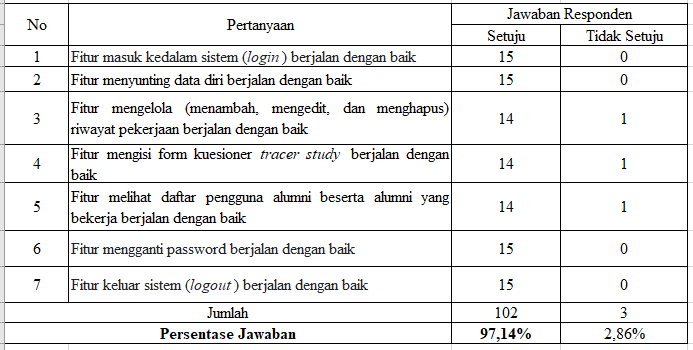
\includegraphics[width=11cm,height=8cm]{gambar/UAT/f_alumni}
		\label{f_alumni}
	\end{table}
	
	%lihat lg hasil real nya/jelasin
	Berdasarkan hasil uji coba fungsional yang dilakukan pada 15 responden alumni, didapatkan jumlah total jawaban 102 dari maksimal nilai 105, maka persentase jawaban adalah \textbf{97.14\%} sehingga dapat dikatakan fitur-fitur pada halaman alumni dapat berjalan dengan baik dan sesuai dengan yang diharapkan. 
	
	\item Uji Coba Kebergunaan
	
	Berikut merupakan daftar pertanyaan uji \textit{usability} pada Alumni:
	
	\begin{table}[H]
		\centering
		\caption{Daftar Pertanyaan Uji \textit{Usability} pada Alumni}
		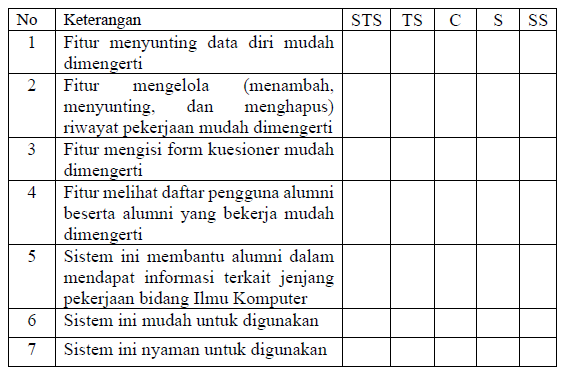
\includegraphics[width=11cm,height=8cm]{gambar/UAT/u_alumni}
		\label{u_alumni}
	\end{table}
	
	Berikut merupakan hasil uji \textit{usability} pada alumni yang dapat dilihat pada tabel berikut:
	
	\begin{table}[H]
		\centering
		\caption{Hasil Uji \textit{Usability} pada Alumni}
		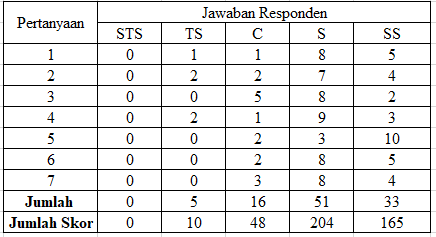
\includegraphics[width=12cm,height=8cm]{gambar/UAT/hasil_u_alumni}
		\label{h_u_alumni}
	\end{table}
	
	$Nilai$ $Total = (0 \times 1) + (5 \times 2) + (16 \times 3) + (51 \times 4) + (33 \times 5) = 427$
		
	$Persentase$ $kelayakan (\%) = \frac{427}{525} $ $\times 100\%$ = 81.33\%
	
	Berdasarkan hasil uji coba kebergunaan yang telah dilakukan pada 15 responden alumni, didapatkan persentase kelayakan senilai \textbf{81.33\%}. Maka dapat dikatakan halaman pada \textit{user} alumni mendapatkan predikat sangat sesuai untuk aspek kebergunaan sistem.
	
\end{enumerate}

\subsection{Pengujian oleh Pengguna Alumni}
\textit{User Acceptance Test} pada \textit{user} Pengguna Alumni dilakukan oleh 5 responden yang merupakan atasan dari alumni di instansi tempat alumni bekerja. Penilaian yang diberikan mengenai fungsionalitas dan kebergunaan dari halaman \textit{user} pengguna alumni pada sistem \textit{tracer study} Ilmu Komputer.

\begin{enumerate}
	\item Uji Coba Fungsional
	
	Tabel 4.10 adalah hasil uji fungsional pada pengguna alumni :
	
	\begin{table}[H]
		\centering
		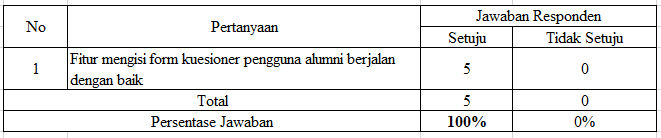
\includegraphics[width=11cm,height=3cm]{gambar/UAT/f_pengguna}
		\caption{Hasil Uji Fungsional pada Pengguna Alumni}
		\label{f_pengguna}
	\end{table}
	
	%lihat lg hasil real nya/jelasin
	Berdasarkan hasil uji coba fungsional yang dilakukan pada \textit{user} pengguna alumni, sistem informasi
	\textit{tracer study} prodi Ilmu Komputer dapat berjalan dengan baik dan sesuai dengan yang diharapkan. Pengguna alumni dapat mengisi kuesioner secara \textit{online}.
	
	\item Uji Coba Kebergunaan
	
	Tabel 4.11 merupakan daftar pertanyaan dari uji kebergunaan/\textit{usability} pada pengguna alumni:
	
	\begin{table}[H]
		\centering
		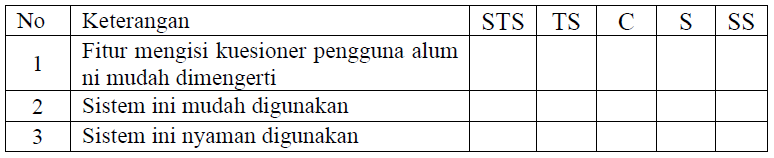
\includegraphics[width=12cm,height=3cm]{gambar/UAT/u_pengguna}
		\caption{Daftar Pertanyaan Uji \textit{Usability} pada Pengguna Alumni}
		\label{u_pengguna}
	\end{table}
	
	Berikut merupakan hasil uji \textit{usability} pada pengguna alumni yang dapat dilihat pada tabel berikut:
	
	\begin{table}[H]
		\centering
		\caption{Hasil Uji \textit{Usability} pada Pengguna Alumni}
		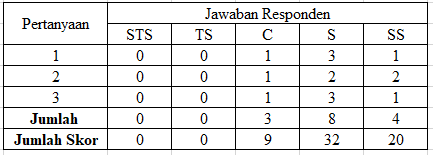
\includegraphics[width=10cm,height=5cm]{gambar/UAT/hasil_u_pengguna}
		\label{h_u_pengguna}
	\end{table}
	
	
	$Nilai$ $Total = (0 \times 1) + (0 \times 2) + (3 \times 3) + (8 \times 4) + (4 \times 5) = 61$
	
	$Persentase$ $kelayakan (\%) = \frac{61}{75} $ $\times 100\%$ = 81.33\%
	
	Berdasarkan hasil uji coba kebergunaan yang telah dilakukan pada 5 responden pengguna alumni, didapatkan persentase kelayakan senilai \textbf{81.33\%}. Maka dapat dikatakan halaman pada \textit{user} pengguna alumni mendapatkan predikat sangat sesuai untuk aspek kebergunaan sistem.
	
\end{enumerate}

%\subsection{Pengujian oleh Ahli}

%Pengujian sistem oleh ahli dilakukan pada keseluruhan sistem. Uji fungsional maupun uji kebergunaan dilakukan pada setiap \textit{user}, yaitu admin, koorprodi, alumni, dan pengguna alumni. Berdasarkan hasil uji coba fungsional yang dilakukan ahli, fungsionalitas sistem pada setiap \textit{user} dapat berjalan dengan baik dan sesuai dengan yang diharapkan. %catatan hasil real
%Hasil uji coba fungsional oleh ahli dapat dilihat sebagai berikut :

%tabel semua fungsional

%Hasil uji coba kualitas yang dilakukan ahli, sistem informasi\textit{tracer study} ilmu komputer dapat berjalan dengan baik dan sudah cukup sesuai dengan kebutuhan. %catatan hasil real
%Hasil uji coba kualitas oleh ahli dapat dilihat sebagai berikut

%tabel semua kualitas

\subsection{Hasil Pengujian Keseluruhan Sistem}
Berdasarkan hasil pengujian fungsional dan kebergunaan (\textit{usability}) Sistem Informasi \textit{Tracer Study} Program Studi Ilmu Komputer pada semua \textit{user},didapatkan bahwa fitur-fitur yang terdapat pada sistem dapat berjalan dengan baik. Selain itu, didapatkan persentase kelayakan sebagai berikut:
 
\begin{itemize}
	\item Halaman \textit{user} Admin : 80\%
	\item Halaman \textit{user} Koorprodi : 100\%
	\item Halaman \textit{user} Alumni : 81.33\%
	\item Halaman \textit{user} Pengguna Alumni : 81.33\%
\end{itemize}

	Dari persentase masing-masing \textit{user} kemudian dihitung total persentase kelayakan yang merupakan rata-rata dari nilai persentase kelayakan semua user, dapat dilihat sebagai berikut:
	
	$Total Persentase Kelayakan (\%) = \frac{80\%+ 100\% + 81.33\%+ 81.33\%}{4} = 85.66\% $
	
	Berdasarkan perhitungan tersebut didapatkan total persentase kelayakan senilai \textbf{85.66\%} berada pada rentang tafsiran 81\%-100\%,  maka dapat dikatakan bahwa nilai kebergunaan pada keseluruhan sistem mendapatkan predikat sangat sesuai. 

% Baris ini digunakan untuk membantu dalam melakukan sitasi
% Karena diapit dengan comment, maka baris ini akan diabaikan
% oleh compiler LaTeX.
\begin{comment}
\bibliography{daftar-pustaka}
\end{comment}